\documentclass[
  shownotes,
  xcolor={svgnames},
  hyperref={colorlinks,citecolor=DarkBlue,linkcolor=DarkRed,urlcolor=DarkBlue}
  , aspectratio=169]{beamer}
\usepackage{animate}
\usepackage{amsmath}
\usepackage{amsfonts}
\usepackage{amssymb}
\usepackage{pifont}
\usepackage{mathpazo}
%\usepackage{xcolor}
\usepackage{multimedia}
\usepackage{fancybox}
\usepackage[para]{threeparttable}
\usepackage{multirow}
\setcounter{MaxMatrixCols}{30}
\usepackage{subcaption}
\usepackage{graphicx}
\usepackage{lscape}
\usepackage[compatibility=false,font=small]{caption}
\usepackage{booktabs}
\usepackage{ragged2e}
\usepackage{chronosys}
\usepackage{appendixnumberbeamer}
\usepackage{animate}
\setbeamertemplate{caption}[numbered]
\usepackage{color}
%\usepackage{times}
\usepackage{tikz}
\usepackage{comment} %to comment
%% BibTeX settings
\usepackage{natbib}
\bibliographystyle{apalike}
\bibpunct{(}{)}{,}{a}{,}{,}
\setbeamertemplate{bibliography item}{[\theenumiv]}

% Defines columns for bespoke tables
\usepackage{array}
\newcolumntype{L}[1]{>{\raggedright\let\newline\\\arraybackslash\hspace{0pt}}m{#1}}
\newcolumntype{C}[1]{>{\centering\let\newline\\\arraybackslash\hspace{0pt}}m{#1}}
\newcolumntype{R}[1]{>{\raggedleft\let\newline\\\arraybackslash\hspace{0pt}}m{#1}}


\usepackage{xfrac}


\usepackage{multicol}
\setlength{\columnsep}{0.5cm}

% Theme and colors
\usetheme{Boadilla}

% I use steel blue and a custom color palette. This defines it.
\definecolor{andesred}{HTML}{af2433}

% Other options
\providecommand{\U}[1]{\protect\rule{.1in}{.1in}}
\usefonttheme{serif}
\setbeamertemplate{itemize items}[default]
\setbeamertemplate{enumerate items}[square]
\setbeamertemplate{section in toc}[circle]

\makeatletter

\definecolor{mybackground}{HTML}{82CAFA}
\definecolor{myforeground}{HTML}{0000A0}

\setbeamercolor{normal text}{fg=black,bg=white}
\setbeamercolor{alerted text}{fg=red}
\setbeamercolor{example text}{fg=black}

\setbeamercolor{background canvas}{fg=myforeground, bg=white}
\setbeamercolor{background}{fg=myforeground, bg=mybackground}

\setbeamercolor{palette primary}{fg=black, bg=gray!30!white}
\setbeamercolor{palette secondary}{fg=black, bg=gray!20!white}
\setbeamercolor{palette tertiary}{fg=white, bg=andesred}

\setbeamercolor{frametitle}{fg=andesred}
\setbeamercolor{title}{fg=andesred}
\setbeamercolor{block title}{fg=andesred}
\setbeamercolor{itemize item}{fg=andesred}
\setbeamercolor{itemize subitem}{fg=andesred}
\setbeamercolor{itemize subsubitem}{fg=andesred}
\setbeamercolor{enumerate item}{fg=andesred}
\setbeamercolor{item projected}{bg=gray!30!white,fg=andesred}
\setbeamercolor{enumerate subitem}{fg=andesred}
\setbeamercolor{section number projected}{bg=gray!30!white,fg=andesred}
\setbeamercolor{section in toc}{fg=andesred}
\setbeamercolor{caption name}{fg=andesred}
\setbeamercolor{button}{bg=gray!30!white,fg=andesred}


\usepackage{fancyvrb}
\newcommand{\VerbBar}{|}
\newcommand{\VERB}{\Verb[commandchars=\\\{\}]}
\DefineVerbatimEnvironment{Highlighting}{Verbatim}{commandchars=\\\{\}}
% Add ',fontsize=\small' for more characters per line
\usepackage{framed}
\definecolor{shadecolor}{RGB}{248,248,248}
\newenvironment{Shaded}{\begin{snugshade}}{\end{snugshade}}
\newcommand{\AlertTok}[1]{\textcolor[rgb]{0.94,0.16,0.16}{#1}}
\newcommand{\AnnotationTok}[1]{\textcolor[rgb]{0.56,0.35,0.01}{\textbf{\textit{#1}}}}
\newcommand{\AttributeTok}[1]{\textcolor[rgb]{0.77,0.63,0.00}{#1}}
\newcommand{\BaseNTok}[1]{\textcolor[rgb]{0.00,0.00,0.81}{#1}}
\newcommand{\BuiltInTok}[1]{#1}
\newcommand{\CharTok}[1]{\textcolor[rgb]{0.31,0.60,0.02}{#1}}
\newcommand{\CommentTok}[1]{\textcolor[rgb]{0.56,0.35,0.01}{\textit{#1}}}
\newcommand{\CommentVarTok}[1]{\textcolor[rgb]{0.56,0.35,0.01}{\textbf{\textit{#1}}}}
\newcommand{\ConstantTok}[1]{\textcolor[rgb]{0.00,0.00,0.00}{#1}}
\newcommand{\ControlFlowTok}[1]{\textcolor[rgb]{0.13,0.29,0.53}{\textbf{#1}}}
\newcommand{\DataTypeTok}[1]{\textcolor[rgb]{0.13,0.29,0.53}{#1}}
\newcommand{\DecValTok}[1]{\textcolor[rgb]{0.00,0.00,0.81}{#1}}
\newcommand{\DocumentationTok}[1]{\textcolor[rgb]{0.56,0.35,0.01}{\textbf{\textit{#1}}}}
\newcommand{\ErrorTok}[1]{\textcolor[rgb]{0.64,0.00,0.00}{\textbf{#1}}}
\newcommand{\ExtensionTok}[1]{#1}
\newcommand{\FloatTok}[1]{\textcolor[rgb]{0.00,0.00,0.81}{#1}}
\newcommand{\FunctionTok}[1]{\textcolor[rgb]{0.00,0.00,0.00}{#1}}
\newcommand{\ImportTok}[1]{#1}
\newcommand{\InformationTok}[1]{\textcolor[rgb]{0.56,0.35,0.01}{\textbf{\textit{#1}}}}
\newcommand{\KeywordTok}[1]{\textcolor[rgb]{0.13,0.29,0.53}{\textbf{#1}}}
\newcommand{\NormalTok}[1]{#1}
\newcommand{\OperatorTok}[1]{\textcolor[rgb]{0.81,0.36,0.00}{\textbf{#1}}}
\newcommand{\OtherTok}[1]{\textcolor[rgb]{0.56,0.35,0.01}{#1}}
\newcommand{\PreprocessorTok}[1]{\textcolor[rgb]{0.56,0.35,0.01}{\textit{#1}}}
\newcommand{\RegionMarkerTok}[1]{#1}
\newcommand{\SpecialCharTok}[1]{\textcolor[rgb]{0.00,0.00,0.00}{#1}}
\newcommand{\SpecialStringTok}[1]{\textcolor[rgb]{0.31,0.60,0.02}{#1}}
\newcommand{\StringTok}[1]{\textcolor[rgb]{0.31,0.60,0.02}{#1}}
\newcommand{\VariableTok}[1]{\textcolor[rgb]{0.00,0.00,0.00}{#1}}
\newcommand{\VerbatimStringTok}[1]{\textcolor[rgb]{0.31,0.60,0.02}{#1}}
\newcommand{\WarningTok}[1]{\textcolor[rgb]{0.56,0.35,0.01}{\textbf{\textit{#1}}}}
\usepackage{graphicx}
\makeatletter

\definecolor{airforceblue}{rgb}{0.36, 0.54, 0.66}

\usepackage{tikz}
% Tikz settings optimized for causal graphs.
\usetikzlibrary{shapes,decorations,arrows,calc,arrows.meta,fit,positioning}
\tikzset{
    -Latex,auto,node distance =1 cm and 1 cm,semithick,
    state/.style ={ellipse, draw, minimum width = 0.7 cm},
    point/.style = {circle, draw, inner sep=0.04cm,fill,node contents={}},
    bidirected/.style={Latex-Latex,dashed},
    el/.style = {inner sep=2pt, align=left, sloped}
}


\makeatother






%%%%%%%%%%%%%%% BEGINS DOCUMENT %%%%%%%%%%%%%%%%%%

\begin{document}
 
\title[Lecture 22]{Lecture 22: \\ Ensembles: Bagging, Random Forests, \& Intro to Boosting}
\subtitle{Big Data and Machine Learning for Applied Economics \\ Econ 4676}
\date{\today}

\author[Sarmiento-Barbieri]{Ignacio Sarmiento-Barbieri}
\institute[Uniandes]{Universidad de los Andes}


\begin{frame}[noframenumbering]
\maketitle
\end{frame}

%%%%%%%%%%%%%%%%%%%%%%%%%%%%%%%%%%%




%----------------------------------------------------------------------% 

\begin{frame}
\frametitle{Agenda}

\tableofcontents

\end{frame}
%----------------------------------------------------------------------%
\section{Recap}
%----------------------------------------------------------------------%

%----------------------------------------------------------------------%
\begin{frame}
\frametitle{CARTs}



\begin{figure}[H] \centering
            \captionsetup{justification=centering}
              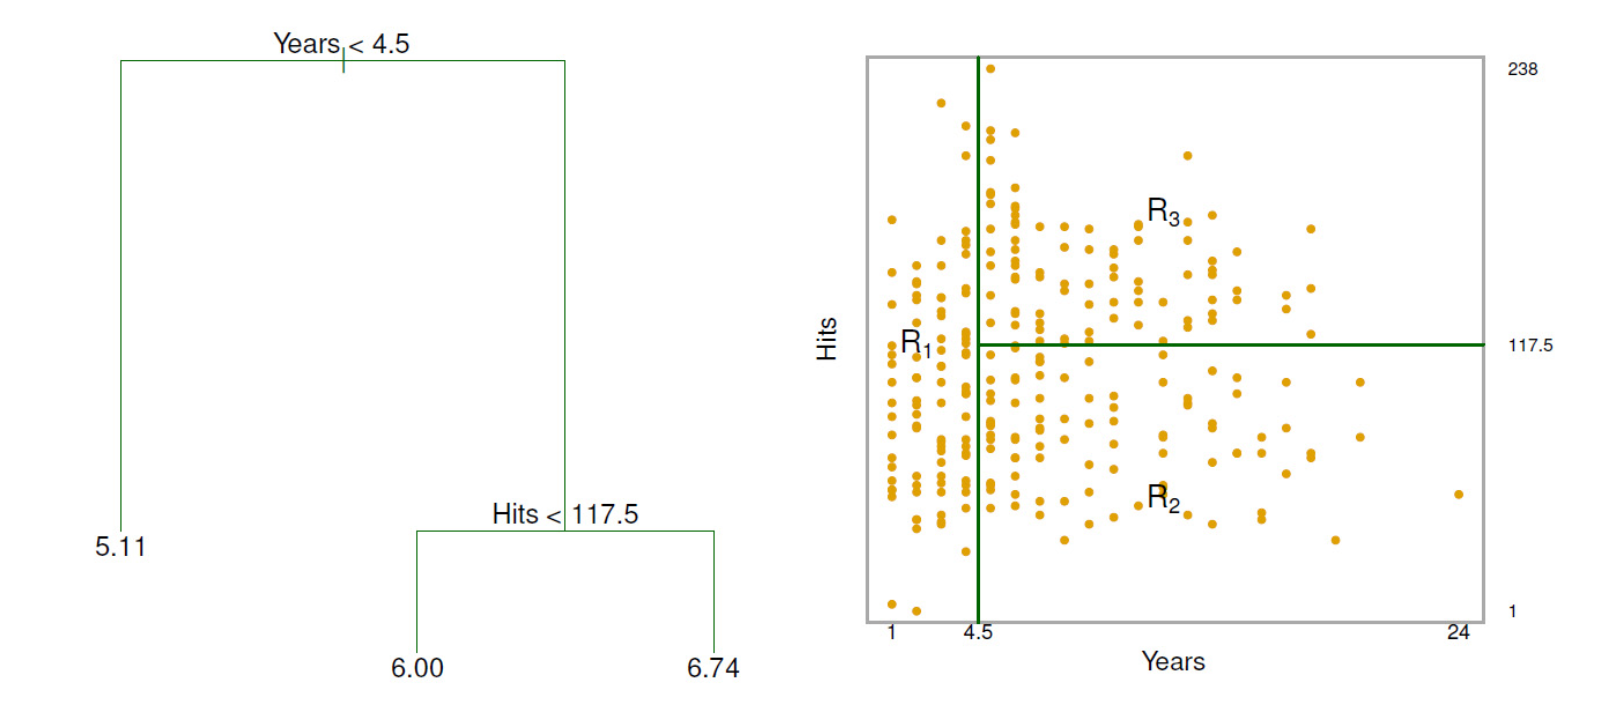
\includegraphics[scale=0.4]{figures/hitters.png}                           
 \end{figure}


\end{frame}
%----------------------------------------------------------------------%
\begin{frame}
\frametitle{CARTs}

\begin{itemize}
  \item Problem then boils down to searching the partition variable $X_j$ and the partition point $s$ such that
    \begin{align}
    \underset{j,s}{min} \left[ \underset{c_1}{min}\sum_{x_i\in R_1(j,s)}(y-c_1)^2+ \underset{c_2}{min}\sum_{x_i\in R_2(j,s)}(y-c_2)^2\right]
    \end{align}

  \item For each partition variable, and partition point, the internal minimization is the mean of each region
  \begin{align}
   \hat{c}_m =\frac{1}{n_m} \sum(y_i|x_i \in R_m)
  \end{align}
  \item Process is repeated inside each region. 
  \pause
  \item If the final tree has M regions then the prediction is 
  \begin{align}
  \hat{f}(x) = \sum_{m=1}^M \hat{c}_m I(x \in R_m)
  \end{align}

\end{itemize}

\end{frame}
%----------------------------------------------------------------------%
\begin{frame}[fragile]
\frametitle{CARTs}

\begin{itemize}
  \item Cost complexity of tree $T$
  \begin{align}
    C_{\alpha}(T)= \sum_{m=1}^{[T]} n_m Q_m (T) + \alpha [T]
  \end{align}

    \begin{itemize}
    \item where $Q_m (T)=\frac{1}{n_m} \sum_{x_i\in R_m} (y_i-\hat{c}_m)^2$ for regression trees
    \medskip
    \item  $Q_m (T)$ penalizes heterogeneity (impurity) within each region, and the second term the number of regions.
    \medskip
    \item  Objective: for a given $\alpha$, find the optimal pruning that minimizes $C_{\alpha}(T)$
    \end{itemize}
\end{itemize}
\end{frame}
%----------------------------------------------------------------------%
\begin{frame}[fragile]
\frametitle{CARTs}

\begin{itemize}
  \item Smart way to represent nonlinearities. Most relevant variables on top.
  \medskip
  \item Very easy to communicate.
  \medskip
  \item  Reproduces human decision-making process.
  \medskip
  \item Trees are intuitive and do OK, but
  \begin{itemize}
    \item They are not very good at prediction 
    \item If the structure is linear, CART does not work well.
    \item  Not very robust
  \end{itemize}
  
\end{itemize}


\end{frame}
%----------------------------------------------------------------------%
\section{Bagging and Random Forests }
%----------------------------------------------------------------------%
\begin{frame}[fragile]
\frametitle{Bagging}

\begin{itemize}
  \item We can improve performance a lot using either bootstrap aggregation (bagging), random forests, or boosting.
  \item Bagging \& Random Forests:
    \begin{itemize}
      \item Repeatedly draw bootstrap samples $(X_i^b,Y_i^b)_{i=1}^N$ from the observed sample.
      \pause
      \item For each bootstrap sample, fit a regression tree $\hat{f}^b(x)$
      \pause
      \item Average across bootstrap samples to get the predictor
      \begin{align}
        \hat{f}_{bag} =\frac{1}{B}\sum_{b=1}^B \hat{f}^b(x)
      \end{align}
\item Basically we are smoothing predictions. 
\item Idea: the variance of the average is less than that of a single prediction.
\end{itemize}

\end{itemize}

\end{frame}

%----------------------------------------------------------------------%
\begin{frame}[fragile]
\frametitle{Bagging}

\begin{figure}[H] \centering
            \captionsetup{justification=centering}
              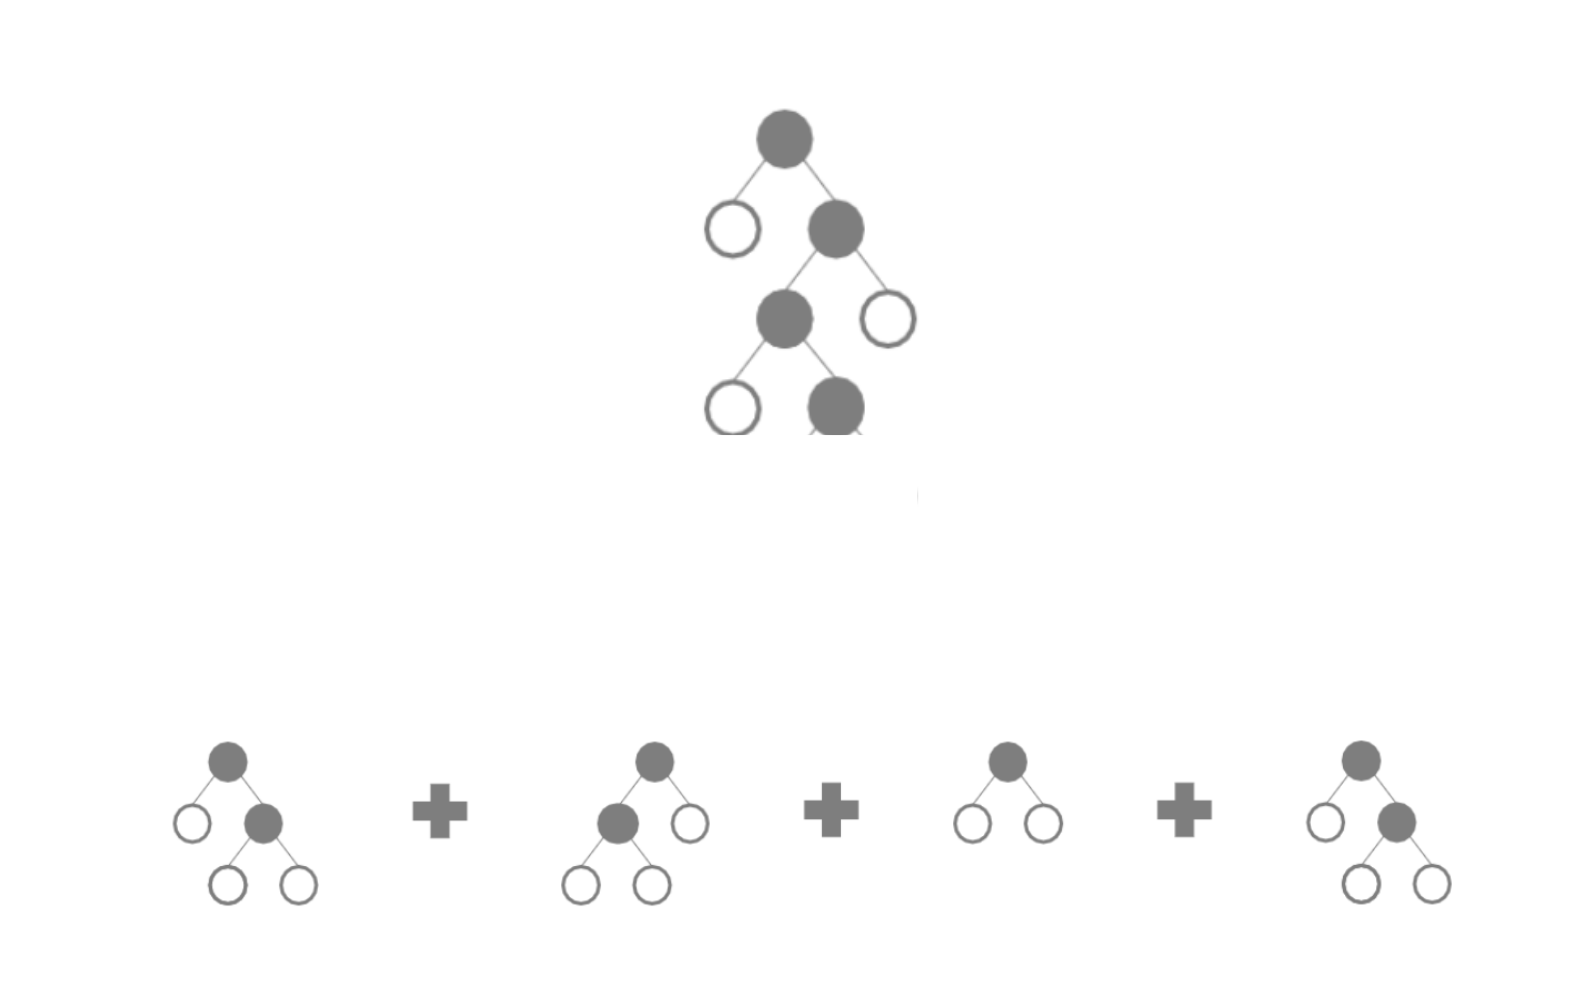
\includegraphics[scale=0.4]{figures/trees_to_forests.png}
 \end{figure}
\end{frame}



%----------------------------------------------------------------------%
\begin{frame}[fragile]
\frametitle{Random Forests}

\begin{itemize}
\item Problem with bagging: if there is a strong predictor, different trees are very similar to each other. High correlation. Is the variance really reduced?
\bigskip
\item Forests: lower the correlation between the trees in the boostrap.
\bigskip
\item If there are $p$ predictors, in each partition use only $m <p$ predictors, chosen randomly
\bigskip
\item Bagging is forest with $m = p$ (use all predictors in each partition).
\bigskip
\item Typically $m = \sqrt(p)$
\end{itemize}

\end{frame}
%----------------------------------------------------------------------%
\begin{frame}[fragile]
\frametitle{Random Forests}

\begin{figure}[H] \centering
            \captionsetup{justification=centering}
              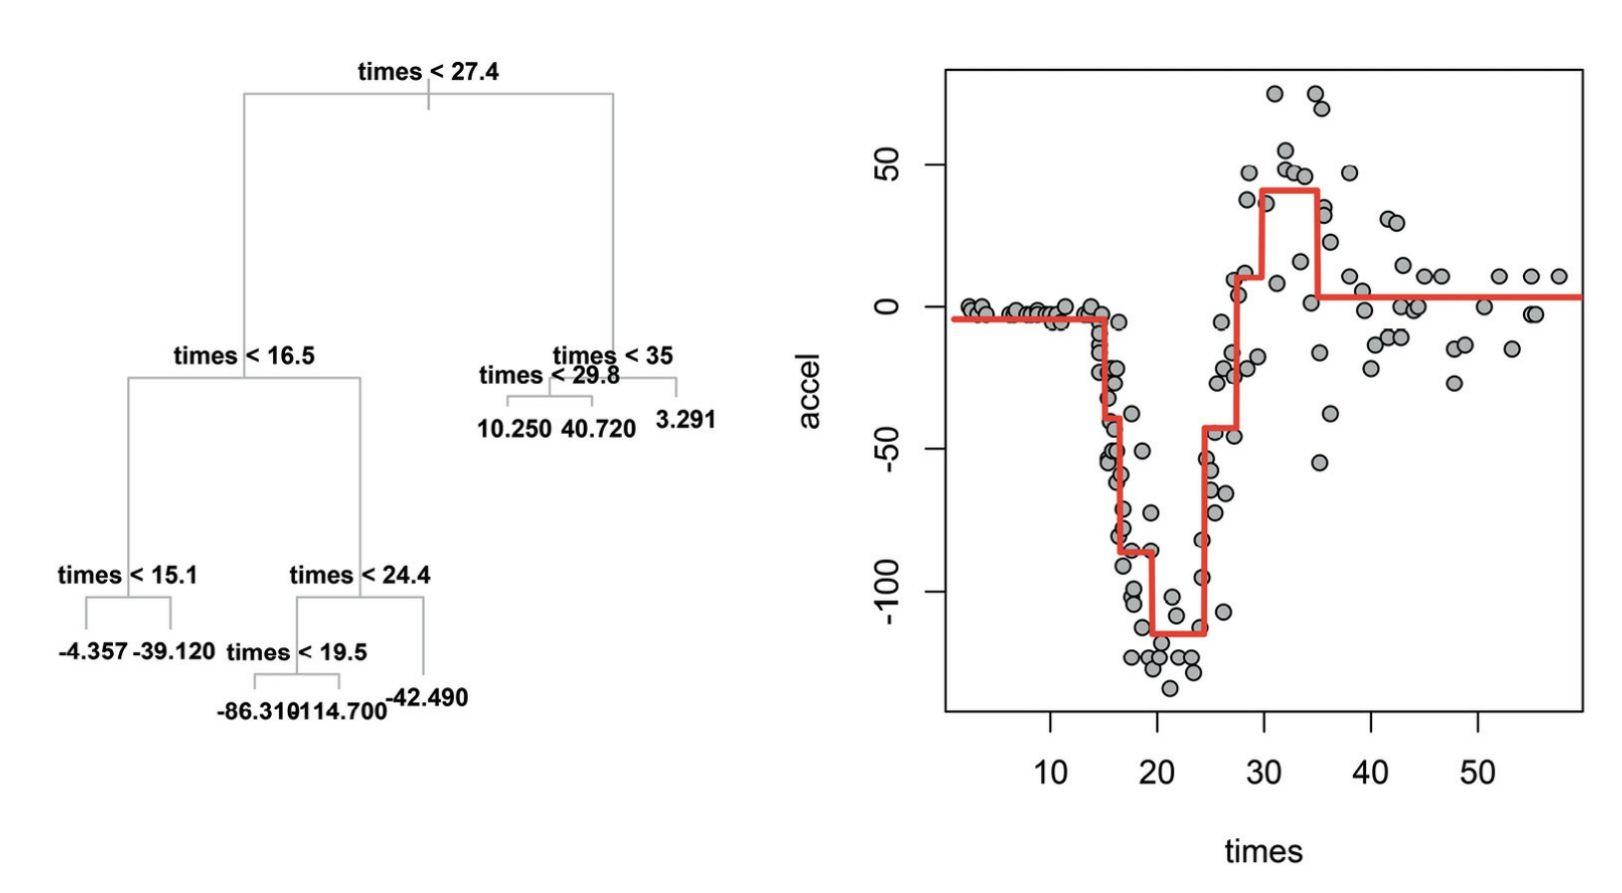
\includegraphics[scale=0.25]{figures/accel_1}
 \end{figure}
\end{frame}

%----------------------------------------------------------------------%
\begin{frame}[fragile]
\frametitle{Random Forests}

\begin{figure}[H] \centering
            \captionsetup{justification=centering}
              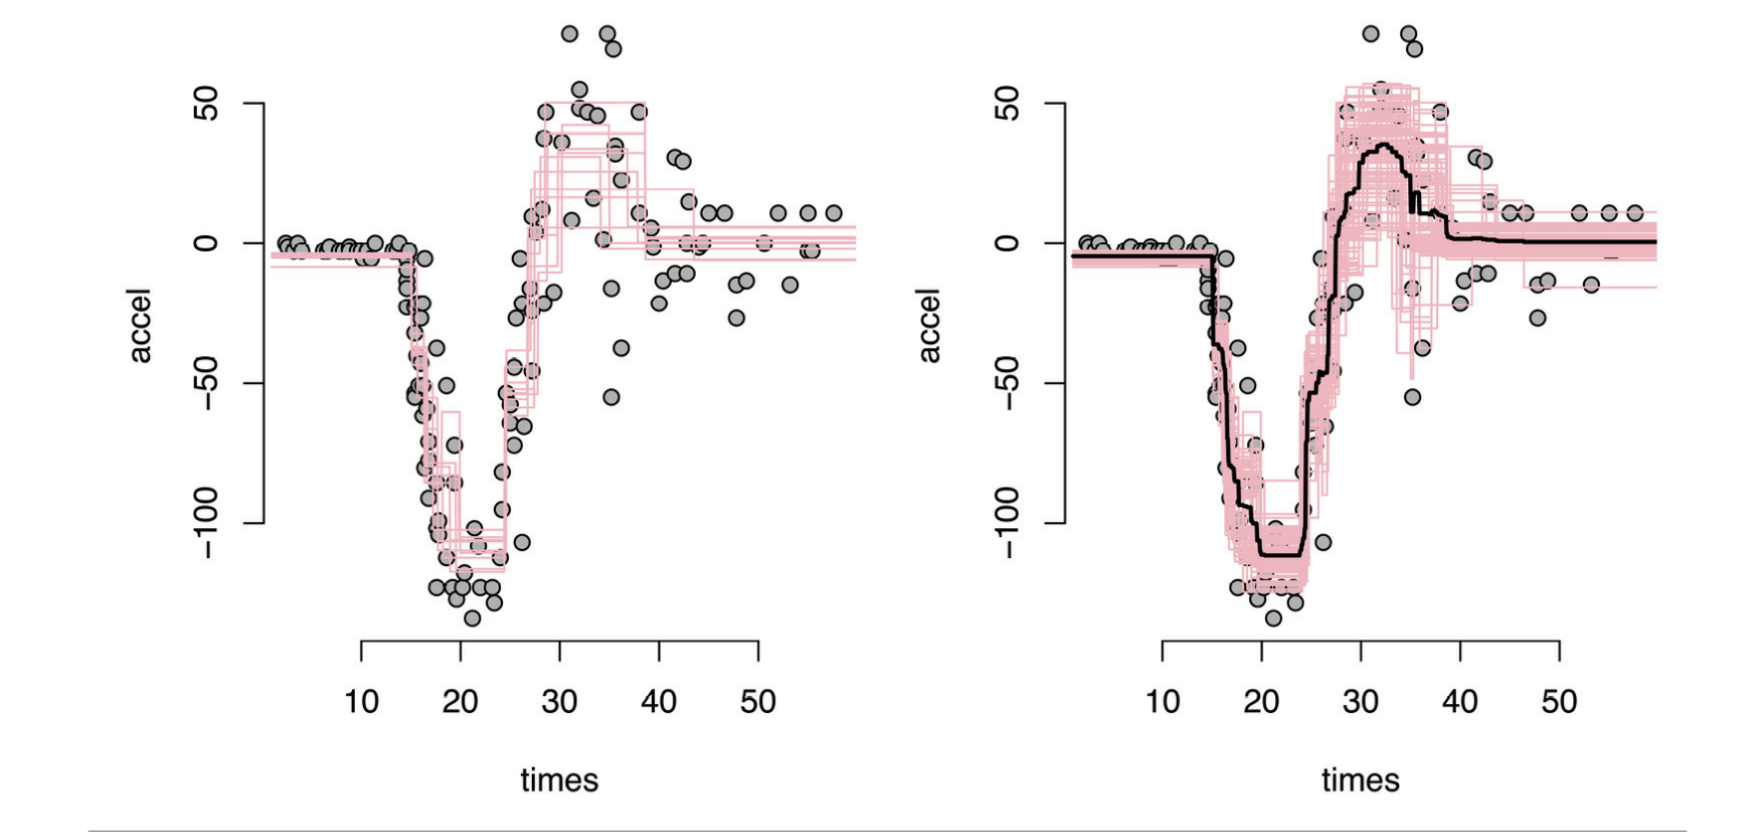
\includegraphics[scale=0.25]{figures/accel_2}
 \end{figure}
\end{frame}

%----------------------------------------------------------------------%
\begin{frame}[fragile]
\frametitle{Random Forests}

\begin{figure}[H] \centering
            \captionsetup{justification=centering}
              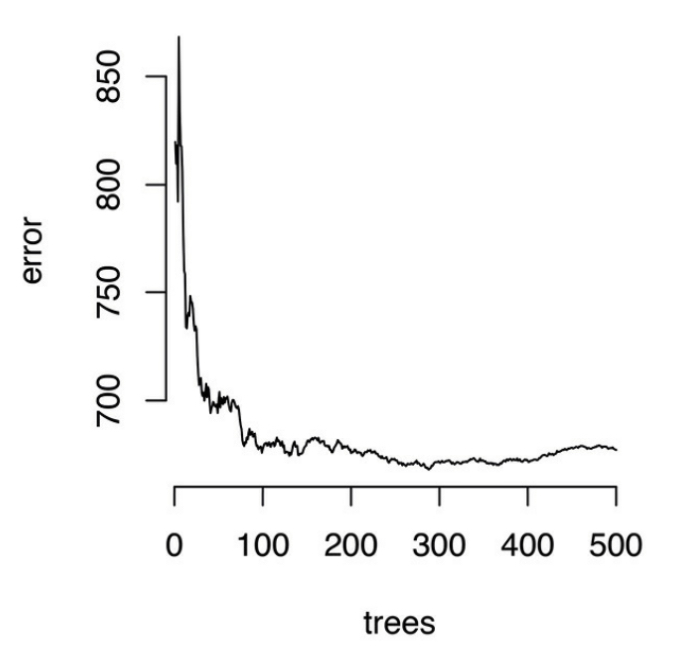
\includegraphics[scale=0.25]{figures/accel_3}
 \end{figure}
\end{frame}



%----------------------------------------------------------------------%
\begin{frame}[fragile]
\frametitle{Random Forests and Trees}
\framesubtitle{Trees}

\begin{scriptsize}
\begin{Shaded}
\begin{Highlighting}[]
\NormalTok{pstcut \textless{}{-}}\StringTok{ }\KeywordTok{prune.tree}\NormalTok{(pstree, }\DataTypeTok{best=}\DecValTok{12}\NormalTok{)}
\KeywordTok{plot}\NormalTok{(pstcut, }\DataTypeTok{col=}\DecValTok{8}\NormalTok{)}
\KeywordTok{text}\NormalTok{(pstcut)}
\end{Highlighting}
\end{Shaded}

\end{scriptsize}
\begin{figure}[H] \centering
            \captionsetup{justification=centering}
              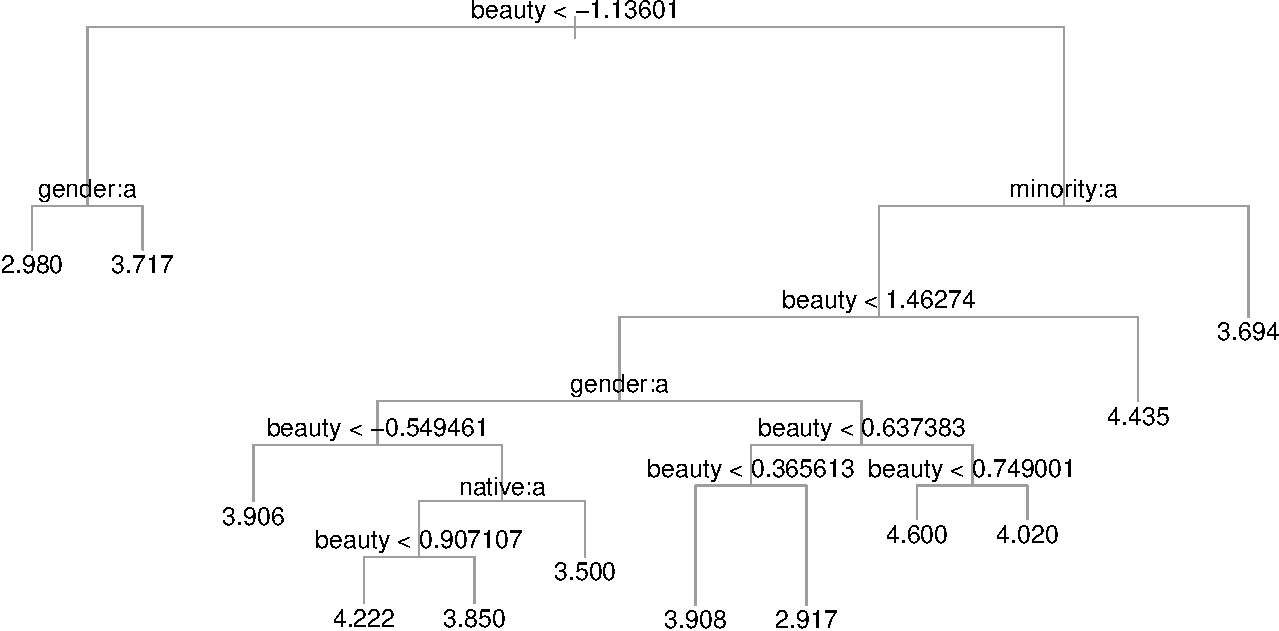
\includegraphics[scale=0.4]{figures/unnamed-chunk-6-1.pdf}              
 \end{figure}


\end{frame}
%----------------------------------------------------------------------%
\begin{frame}[fragile]
\frametitle{Random Forests and Trees}

\begin{Shaded}
\begin{Highlighting}[]
\KeywordTok{require}\NormalTok{(}\StringTok{"ranger"}\NormalTok{)}

\NormalTok{rf\_tree \textless{}{-}}\StringTok{ }\KeywordTok{ranger}\NormalTok{(eval }\OperatorTok{\textasciitilde{}}\NormalTok{beauty }\OperatorTok{+}\StringTok{ }\NormalTok{gender }\OperatorTok{+}\StringTok{ }\NormalTok{minority }\OperatorTok{+}\StringTok{ }\NormalTok{native }\OperatorTok{+}
        \StringTok{ }\NormalTok{tenure }\OperatorTok{+}\StringTok{ }\NormalTok{division, }\DataTypeTok{data=}\NormalTok{tr, }
        \DataTypeTok{write.forest=}\OtherTok{TRUE}\NormalTok{,}\DataTypeTok{num.tree=}\DecValTok{200}\NormalTok{,}\DataTypeTok{min.node.size=}\DecValTok{25}\NormalTok{,}
        \DataTypeTok{importance=}\StringTok{"impurity"}\NormalTok{)}
\KeywordTok{sort}\NormalTok{(rf\_tree}\OperatorTok{$}\NormalTok{variable.importance, }\DataTypeTok{decreasing =} \OtherTok{TRUE}\NormalTok{)}
\end{Highlighting}
\end{Shaded}

\begin{verbatim}
##    beauty  minority    gender    native    tenure  division 
## 22.881176  3.089366  2.608295  2.104095  2.062075  1.627261
\end{verbatim}

\end{frame}

%----------------------------------------------------------------------%
\section{Comparisons: Lasso, CART, Random Forests}
%----------------------------------------------------------------------%
\begin{frame}[fragile]
\frametitle{Comparisons: Lasso, CART, Random Forests}
\frametitle{In sample residuals}


\begin{figure}[H] \centering
            \captionsetup{justification=centering}
              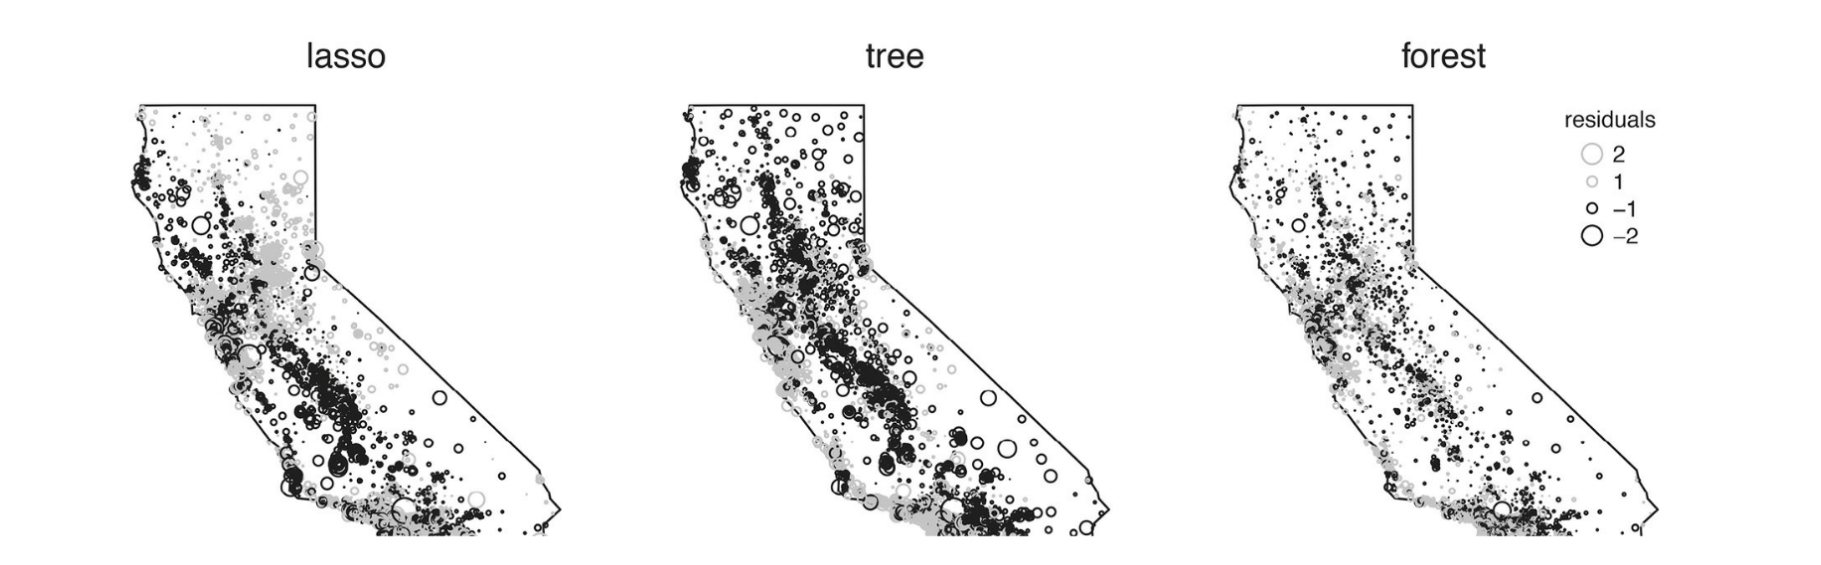
\includegraphics[scale=0.25]{figures/california}
 \end{figure}

\begin{tiny}
\begin{Shaded}
\begin{Highlighting}[]
\CommentTok{\# Model Matrix for Lasso}
\NormalTok{XXca \textless{}{-}}\StringTok{ }\KeywordTok{model.matrix}\NormalTok{(logMedVal}\OperatorTok{\textasciitilde{}}\NormalTok{.}\OperatorTok{*}\NormalTok{longitude}\OperatorTok{*}\NormalTok{latitude, }
      \DataTypeTok{data=}\KeywordTok{data.frame}\NormalTok{(}\KeywordTok{scale}\NormalTok{(CAhousing)))[,}\OperatorTok{{-}}\DecValTok{1}\NormalTok{]}
\end{Highlighting}
\end{Shaded}
\end{tiny}

\end{frame}

%----------------------------------------------------------------------%
\begin{frame}[fragile]
\frametitle{Comparisons: Lasso, CART, Random Forests}
\frametitle{Out of sample MSE}


\begin{figure}[H] \centering
            \captionsetup{justification=centering}
              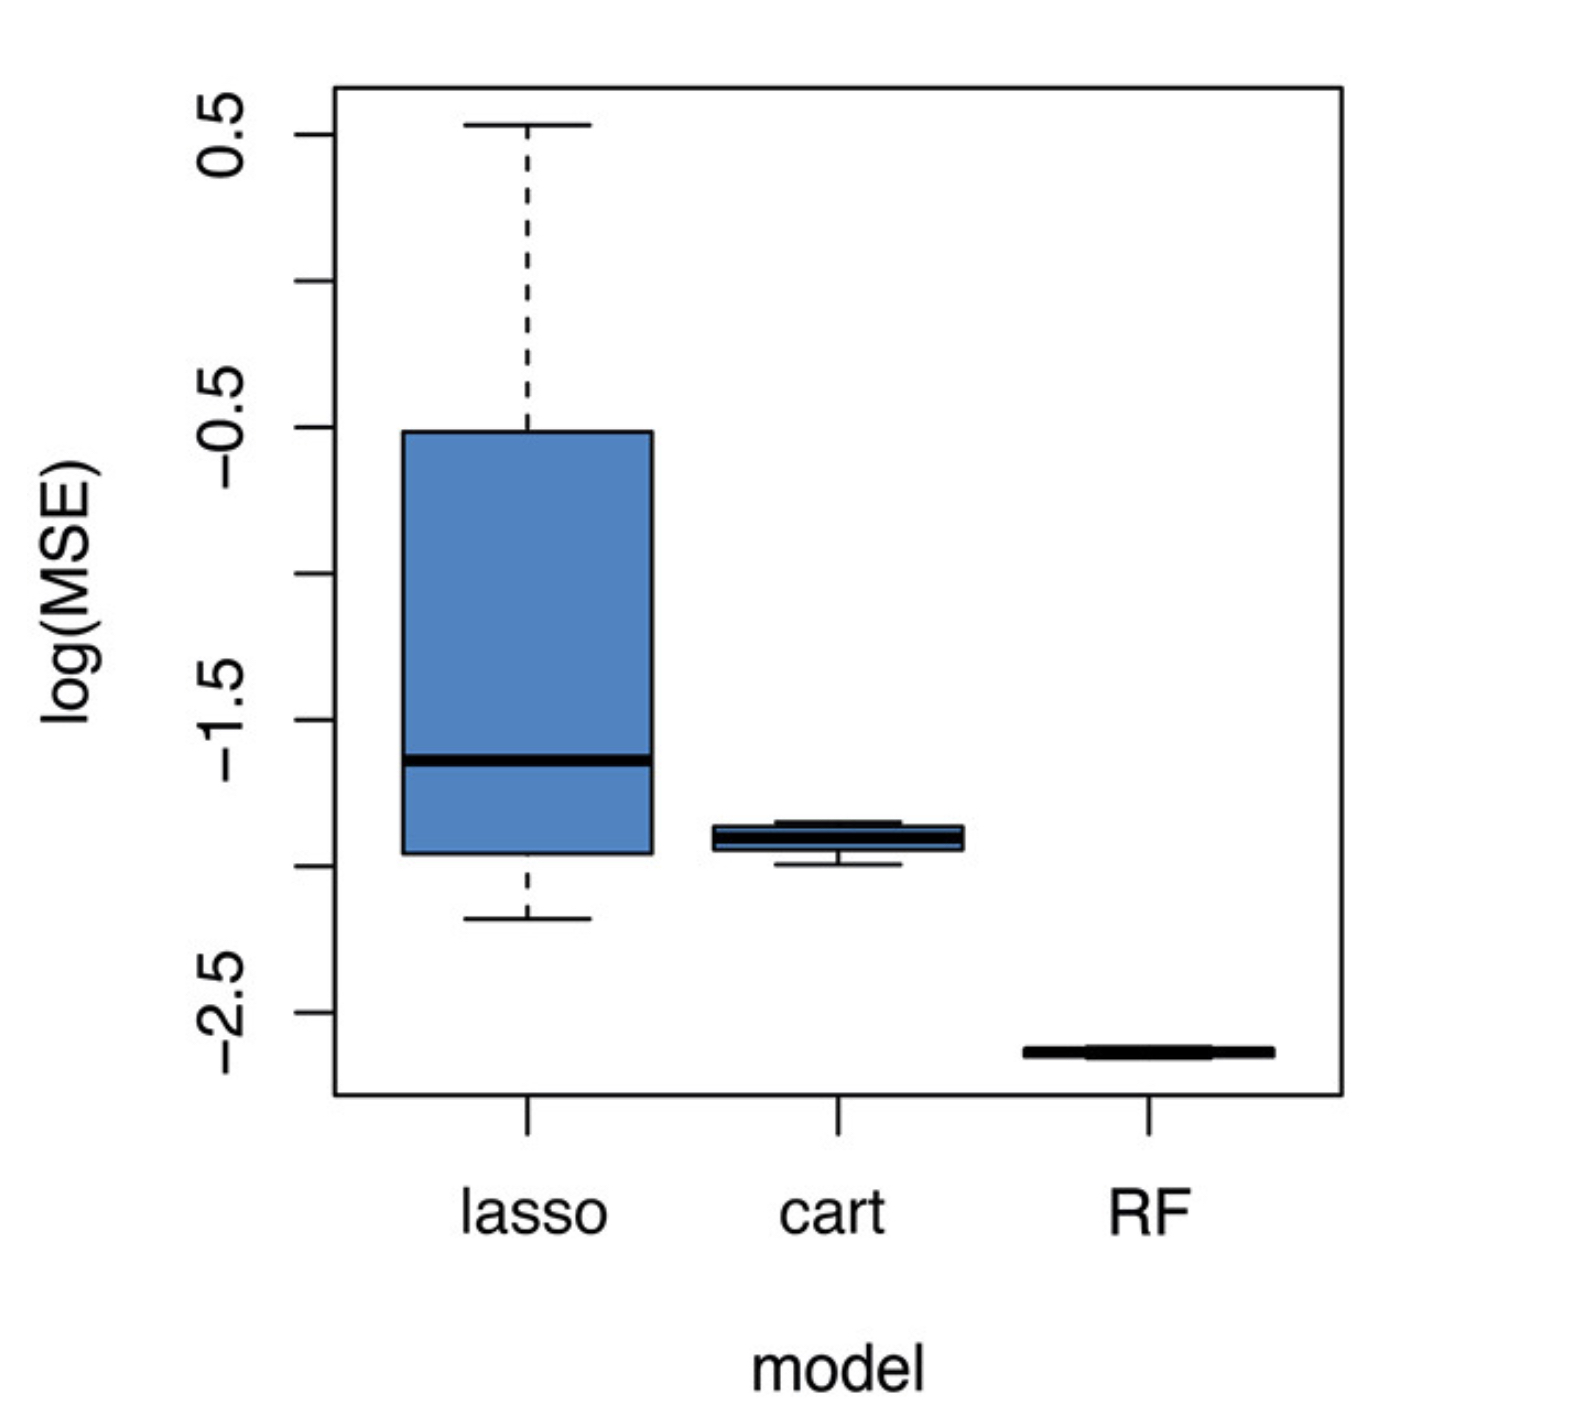
\includegraphics[scale=0.15]{figures/california_out_of_sample}
 \end{figure}

\end{frame}


%----------------------------------------------------------------------%

%----------------------------------------------------------------------%
\section{Boosting}
%----------------------------------------------------------------------%
\begin{frame}[fragile]
\frametitle{Boosting}

\begin{itemize}
\item Problem with CART: high variance. Instability
\medskip
\item Weak classifier: marginally better classifier than flipping a coin (error rate slightly better than .5)
\medskip
\item E.g.: CART with few branches ('stump', two branches)
\medskip
\item Boosting: weighted average of a succession of weak classifiers.
\medskip
\item Vocab
\medskip
  \begin{itemize}
  \item $y \in {-1,1}$ (for simplicity), $X$ vector of predictors.
  \medskip
  \item $y = G (X)$ (classifier)
  \medskip
  \item $err = \frac{1}{N} \sum_{i}^N I(y_i\neq G(x_i))$
  \end{itemize}
\end{itemize}


\end{frame}

%----------------------------------------------------------------------%
\subsection{AdaBoost}
%----------------------------------------------------------------------%
\begin{frame}[fragile]
\frametitle{AdaBoost}
\begin{enumerate}
\item Start with weights $w_i = 1 / N$
\item For m = 1 through M:
\begin{enumerate}
    \item Adjust $G_m(x)$ using weights $w_i$ .
    \item Compute prediction 
    \begin{align}
    err_m = \frac{\sum_{i=1}^N  I(y_i \neq G_m(x_i))}{\sum_{i=1}^N w_i}
    \end{align}
    \item Compute $\alpha_m= ln \left[\frac{(1 - err_m )}{ err_m} \right]$
    \item Update weights: $w_i \leftarrow w_i c_i$ 
    \begin{align}
    c_i = exp \left[\alpha_m  I (y i \neq G_m (x_i )) \right]
    \end{align}
    
\end{enumerate}
\item Output: $G(x) = sgn[\sum_{m = 1}^M \alpha_m G_m(x)]$
\end{enumerate}

\end{frame} 
%----------------------------------------------------------------------%
\begin{frame}[fragile]
\frametitle{AdaBoost}

\begin{itemize}
\item $c_i = exp \left[ \alpha_m I(y_i \neq G_m (x_i )) \right]$
\medskip
\item If it was correctly predicted, $c_i = 1$. No issue.
\medskip
\item Otherwise, $c_i = exp (\alpha_m ) = \frac{(1 - err_m ) }{err_m} > 1$ 
\medskip
\item At each step the method gives more relative importance to the predictions that where wrong.
\medskip
\item Final step: weighted average of predictions at each step.
\end{itemize}
\end{frame}
%----------------------------------------------------------------------%
\begin{frame}[fragile]
\frametitle{AdaBoost}


\begin{figure}[H] \centering
            \captionsetup{justification=centering}
              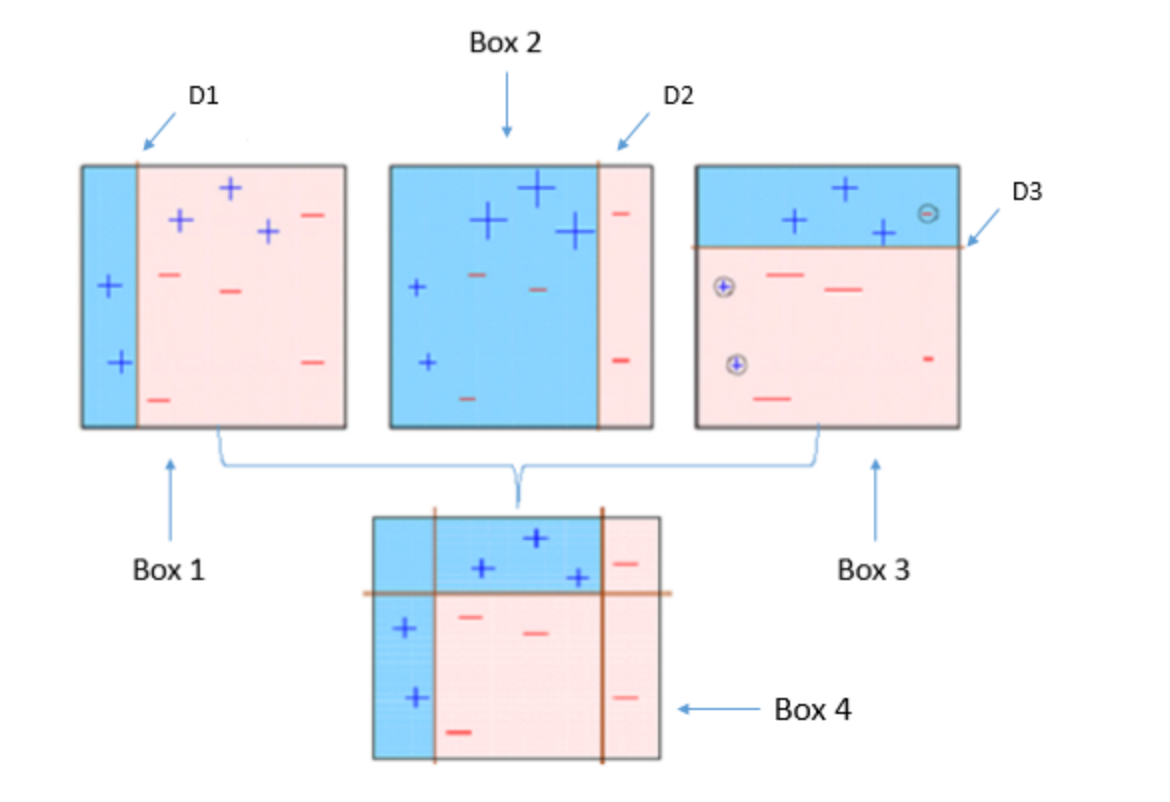
\includegraphics[scale=0.5]{figures/adaboost.png}
              \\
              \tiny
              Source: \url{https://www.analyticsvidhya.com/blog/2015/11/quick-introduction-boosting-algorithms-machine-learning/}
 \end{figure}


\end{frame}

%----------------------------------------------------------------------%
\subsection{Causal Forests}
%----------------------------------------------------------------------%
\begin{frame}[fragile]
\frametitle{Causal Forests}

\begin{figure}[H] \centering
            \captionsetup{justification=centering}
              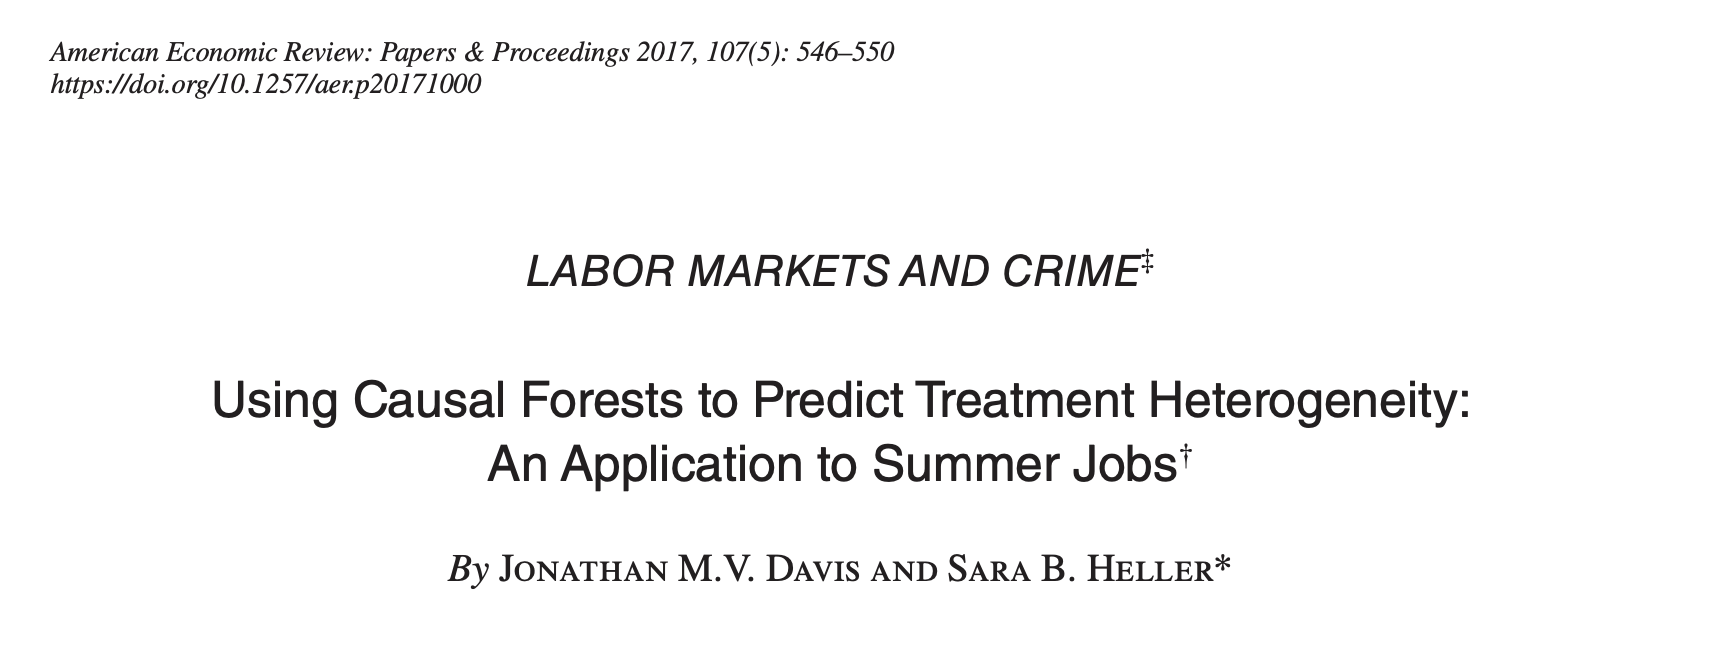
\includegraphics[scale=0.5]{figures/tress_summer_jobs}
              \\
            
 \end{figure}

\end{frame}


%----------------------------------------------------------------------%

\begin{frame}[fragile]
\frametitle{Idle hands are the devil's workshop}

\begin{itemize}

  \item The application uses two large scale RCTs of Chicago's One Summer Plus (OSP) program conducted in 2012 and 2013. OSP provides disadvantaged youth ages 14 to 22 with 25 hours a week of employment, an adult mentor, and some other programming. 
  \medskip
  \item Participants are paid Chicago's minimum wage (\$8.25 at the time). 
  \medskip
  \item Find  a 43 percent reduction in violent crime arrests in the 16 months after random assignment. 

\end{itemize}




\end{frame}

%----------------------------------------------------------------------%
\begin{frame}[fragile]
\frametitle{Causal Tree: Theory Details}



\begin{itemize}
  \item Work well in RCTs
  \medskip
  \item Issue: we do not observe the ground truth
  \medskip
  \item Honest estimation (Innovation):
    \begin{itemize}
      \item One sample to choose partition 
      \medskip
      \item One sample to estimate leaf effects
      \medskip
    \end{itemize}
  \item Why is the split critical?
  \medskip
  \item Fitting both on the training sample risks overfitting: Estimating many “heterogeneous effects” that are really just noise idiosyncratic to the sample.
  \medskip
  \item We want to search for true heterogeneity, not noise
\end{itemize}

\end{frame}


%----------------------------------------------------------------------%
\begin{frame}[fragile]
\frametitle{Heterogeneous Treatment Effects Assumptions}

\begin{itemize}
  \item There are  a couple of assumptions that are key


  \item Assumption 1: Unconfoundedness
  \begin{align}
  Y_i(1), Y_i(0) \perp W_i \ | \ X_i
  \end{align}
  \begin{itemize}
  \item The \emph{unconfoundedness} assumption states that, once we condition on observable characteristics, the treatment assignment is independent to
  how each person would respond to the treatment. 
  \item i.e.,  the rule that determines whether or not a person is treated is determined completely by their observable characteristics. 
  \item This allows, for example, for experiments where people from different genders get treated with different probabilities, 
  \item {\bf rules out} experiments where people self-select into treatment due to some characteristic that is not observed in our data.

\end{itemize}


\end{itemize}




\end{frame}
%----------------------------------------------------------------------%
\begin{frame}[fragile]
\frametitle{Heterogeneous Treatment Effects}

\begin{itemize}
  \item Assumption 2: Overlap
  \medskip
  \begin{align}
  \forall \ x \in \text{supp}\ (X), \qquad 0 < P\ (W = 1 \ | \ X = x)  < 1
  \end{align}

    \begin{itemize}
    \item The \emph{overlap} assumption states that at every point of the covariate space we can always find treated and control individuals.
    \medskip
    \item  i.e., in order to estimate the treatment effect for a person with particular  characteristics \(X_{i} = x\), we need to ensure that we are able to
    observe treated and untreated people with those same characteristics so that we can compare their outcomes. 
    \end{itemize}
\end{itemize}

\end{frame}
%----------------------------------------------------------------------%
\begin{frame}[fragile]
\frametitle{The Honest Target: Athey and Imbens Innovation}


\begin{itemize}
\item The ultimate goal is to construct and assess an algorithm $\pi(.)$ that maximizes the honest criterion

\medskip
\begin{align}
max\,Q^{H}(\pi)=-E_{S^{te},S^{est},S^{tr}}\left[MSE_{\mu}(S^{te},S^{est},S^{tr},\pi(S^{tr})\right]
\end{align}


\item In CART the target is different (adaptive target)
\medskip
\begin{align}
max\,Q^{C}(\pi)=-E_{S^{te},S^{tr}}\left[MSE_{\mu}(S^{te},S^{tr},\pi(S^{tr})\right]
\end{align}


\end{itemize}

\end{frame}
%----------------------------------------------------------------------%
\begin{frame}[fragile]
\frametitle{From Causal Trees to Causal Forest}


The implementation steps are as follows in Davis and Heller (2017):
\medskip
\begin{itemize}


\item (1) Draw a subsample b without replacement containing $n_b = 0.2N$ observations from the N observations in the dataset
\medskip
\item (2) Randomly split the $n_b$ observations in half to form a training sample (tr) and an estimation sample (e) such that $n_{tr}=n_e=\frac{n_b}{2}$. Using just the training sample, start with a single leaf containing all $n_{tr}$ observations.

\end{itemize}

\end{frame}
%----------------------------------------------------------------------%
\begin{frame}[fragile]
\frametitle{From Causal Trees to Causal Forest}


The implementation steps are as follows in Davis and Heller (2017):
\medskip
\begin{itemize}


\item (3) For each value of each covariate, $X_j = x$, form candidate splits of the observations into two groups based on whether $X_j \leq x$. Consider only splits where there are at least ten treatment and ten control observations in both new leaves. 
\item Choose the single split that maximizes an objective function $O$ capturing how much the treatment effect estimates vary across the two resulting subgroups, with a penalty for within leaf variance . If this split increases $O$ relative to no split, implement it and repeat this step in both new leaves. If no split increases O, this is a terminal leaf.

\begin{align}
O = (n_T + n_C)\hat{\tau}^2_l - 2 \left(\frac{\hat{Var}(Y_{Tl})}{n_T}+\frac{\hat{Var}(Y_{Cl})}{n_C}\right)
\end{align}
\medskip

\end{itemize}
\end{frame}
%----------------------------------------------------------------------%
\begin{frame}[fragile]
\frametitle{From Causal Trees to Causal Forest}

\begin{itemize}

\item (4) Once no more splits can be made in step 3, the tree is defined for subsample b. Move to the estimation sample, and group the ne observations into the same tree based on their Xs.
\medskip

\item (5) Using just the estimation sample, calculate $\hat{\tau}=\bar{y}_{Tl}-\bar{y}_{Tc}$ within each terminal leaf. This step makes the tree honest, since treatment effect estimates are made using different observations than the ones that determined the splits.
\medskip

\item (6) Return to the full sample of N observations. Assign $\hat{\tau}_{l,b}=\hat{\tau_l}$ to each observation whose Xs would place it in leaf l, and save this prediction.
\medskip
\item (7) Repeat steps (i) to (vi) B = 25, 000 times


\end{itemize}
\end{frame}
%----------------------------------------------------------------------%
\begin{frame}[fragile]
\frametitle{From Causal Trees to Causal Forest}

\begin{itemize}

  \item Define observation i’s predicted CATE as $\hat{\tau}^{CF}_i (x)=\frac{1}{B} \sum \hat{\tau}_{l,b} $
  \medskip
  \pause
  \item The procedure requires the researcher to select three parameters: the number of trees, the minimum number of treatment and control observations in each leaf, and the subsample size. 
  \medskip
  \item In the absence of formal criteria to guide our choices, we used a large number of trees (more trees reduce the Monte Carlo error introduced by subsampling; we found moving from 10,000 to 25,000 improved the stability of estimates across samples). 
  \medskip
  \begin{itemize}
    \item Increasing the minimum number of observations in each leaf trades off bias and variance; bigger leaves make results more consistent across different samples but predict less heterogeneity. 
    \item Smaller subsamples reduce dependence across trees but increase the variance of each estimate (larger subsamples made little difference in our application).
  \end{itemize}
\end{itemize}

\end{frame}
%----------------------------------------------------------------------%
\begin{frame}[fragile]
\frametitle{From Causal Trees to Causal Forest}

\begin{itemize}


\item We run the entire CF procedure using only $S_{in}$, then use the trees grown in  $S_{in}$ to generate predictions for all observations in  $S_{in}$ and  $S_{out}$.
\medskip
 \item This allows  to assess the performance of the predictions in a hold-out sample (albeit with reduced statistical power) and to check whether heterogeneity is more distinct in  $S_{in}$ than  $S_{out}$, which could be a sign of overfitting.
 \item 
Within each sample, we group youth by whether they are predicted to have a positive or negative treatment effect ($\hat{\tau}^{CF}_i>0$ is desirable for employment and adverse for arrests).
\item  We estimate separate treatment effects for these two subgroups by regressing each outcome on the indicator:

\begin{align}
y_{ib} = \beta_1 I[\hat{\tau}^{CF}_i>0] + \beta_2 T_i I[\hat{\tau}^{CF}_i>0] + \beta_3 T_i \left(1-I[\hat{\tau}^{CF}_i>0] \right)+ X\theta + \alpha_b + u_{ib}
\end{align}

\end{itemize}
\end{frame}
%----------------------------------------------------------------------%
\begin{frame}[fragile]
\frametitle{Causal Forests}

\begin{figure}[H] \centering
            \captionsetup{justification=centering}
              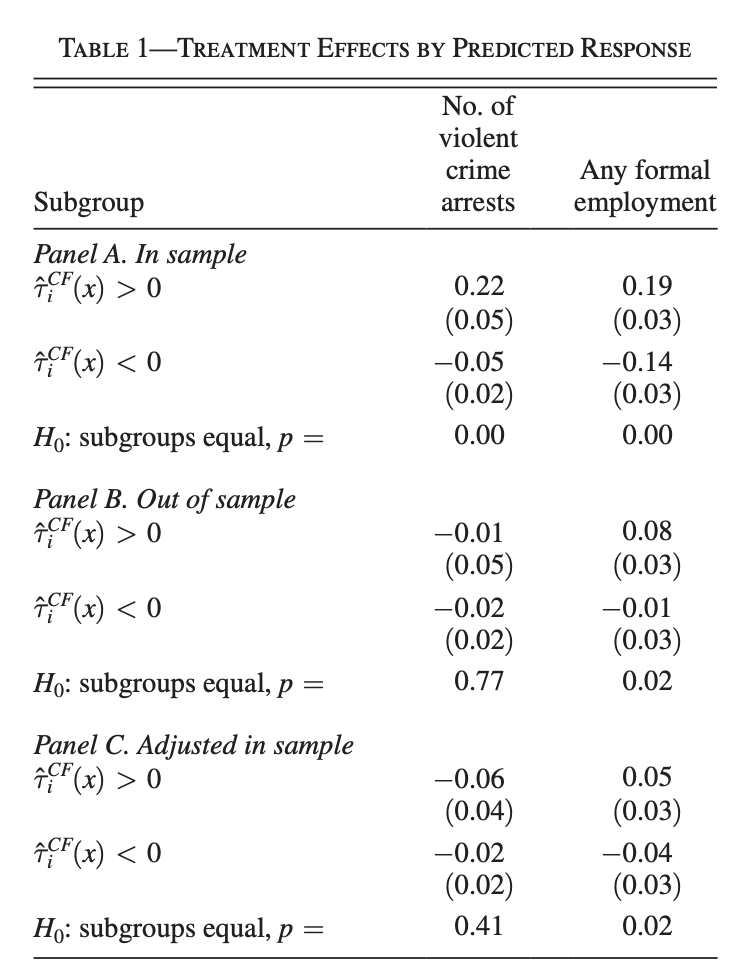
\includegraphics[scale=0.4]{figures/results_aer_trees.png}
              \\
            
 \end{figure}

\end{frame}

%----------------------------------------------------------------------%
\section{Review
 \& Next Steps}
%----------------------------------------------------------------------%
\begin{frame}
\frametitle{Review \& Next Steps}
  
\begin{itemize} 
    \item Bagging and Random Forests
    \medskip
    \item Comparisons: Lasso, CART, Random Forests
    \medskip
    \item AdaBoost
    \medskip
    \item Causal Forests

    \bigskip  
  \item  Next class:  More on boosting


\bigskip  
\item Questions? Questions about software? 

\end{itemize}
\end{frame}
%----------------------------------------------------------------------%
\section{Further Readings}
%----------------------------------------------------------------------%
\begin{frame}
\frametitle{Further Readings}

\begin{itemize}

  \item Athey, S., \& Imbens, G. (2016). Recursive partitioning for heterogeneous causal effects. Proceedings of the National Academy of Sciences, 113(27), 7353-7360.
  \medskip
  \item Davis, Jonathan M.V., and Sara B. Heller. 2017. "Using Causal Forests to Predict Treatment Heterogeneity: An Application to Summer Jobs." American Economic Review, 107 (5): 546-50. 
  \medskip
  \item Friedman, J., Hastie, T., \& Tibshirani, R. (2001). The elements of statistical learning (Vol. 1, No. 10). New York: Springer series in statistics.
  \medskip
  \item Green, D. P., \& Kern, H. L. (2012). Modeling heterogeneous treatment effects in survey experiments with Bayesian additive regression trees. Public opinion quarterly, 76(3), 491-511.
  \medskip
  \item James, G., Witten, D., Hastie, T., \& Tibshirani, R. (2013). An introduction to statistical learning (Vol. 112, p. 18). New York: springer.
  \medskip
  \item Taddy, M. (2019). Business data science: Combining machine learning and economics to optimize, automate, and accelerate business decisions. McGraw Hill Professional.
  

  
\end{itemize}

\end{frame}





%----------------------------------------------------------------------%
%----------------------------------------------------------------------%
\end{document}
%----------------------------------------------------------------------%
%----------------------------------------------------------------------%

